\documentclass{article}
\usepackage{graphicx}
\usepackage[dvipsnames]{xcolor}
\usepackage{fancyvrb}
% \usepackage[legalpaper, landscape, margin=2in]{geometry}
\usepackage{geometry}
 \geometry{
 a4paper,
 total={170mm,257mm},
 left=20mm,
 top=20mm,
 }
 
 
\title {Reviewing Crowdsourcing literature in User Interface Design - Using LISC package }
\author{Sanaz Nabavian}
\begin{document}
\maketitle

\begin{abstract} % abstract
The size and growing scale of the scientific literature result in a time-consuming manual process and limited scope literature summarization methods. These methods, including meta-analyses and systematic reviews, could be an excellent start to find the gap in any area. As a Ph.D. student, I should search for a vast amount of literature to find my topic of interest. I will use the package called LISC in this report for my research area, crowdsourcing, to find the recent two-year research focus. It takes the keywords you are aiming to search, using APIs(application programming interfaces) to collect data from different databases and save the results in defined objects.
\end{abstract}


\section{Introduction}
LISC is an interface using APIs  connected to Pubmed database, providing access to collect and analyze biomedical literature, and to the OpenCitations database (Heibi,et al., 2019), providing access to citation data (Donoghue, 2019). LISC offers Three types of literature data collection: Counts, Words, and Citations(Donoghue, 2019). In this report, I will use this package to find a general understanding of the literature in my area of interest, designing a user interface for a crowdsourcing website.

\section{Method}
\subsection*{Supported API}
Entrez Programming Utilities (E-utilities)
It consists of nine server-side programs that provide an interface to the Entrez query and database system at the National Center for Biotechnology Information (NCBI).  These server-side programs are: 1- EInfo (database statistics), 2- ESearch (text searches), 3- EPost (UID uploads), 4- ESummary (document summary downloads), 5- EFetch (data record downloads), 6-ELink (Entrez links), 7- EGQuery (global query), 8- ESpell (spelling suggestions), 9- ECitMatch (batch citation searching in PubMed)To access these data, a piece of software first posts an E-utility URL to NCBI Then, it retrieves the results of this posting, after which it processes the data as required. The software can thus use any computer language that can send a URL to the E-utilities server and interpret the XML response("National Center for Biotechnology Information", n.d.).
Open Citations
OpenCitations is an independent infrastructure organization for open scholarship dedicated to the publication of open bibliographic and citation data by the use of Semantic Web (Linked Data) technologies. It is also engaged in advocacy for open citations, particularly in its role as a key founding member of the Initiative for Open Citations (I4OC) ("Open Citations," n.d.).
\subsection*{Data collection}
LISC currently offers the following types of literature data collection: 
\newline• Counts: tools to collect and analyze data on the co-occurrence of specified search terms 
\newline• Words: tools to collect and analyze text and meta-data from scientific articles 
\newline• Citations: tools to collect and analyze citation and reference data 

Here, we will use counts object for analyzing the number of co-occurrence of the search keywords. Then, using the word object and analysis to see the new research from 2018.
My research area is about crowdsourcing data, and how the user interface design can change the data quality. So I have entered these keywords and their synonyms as the input of this package. 
\begin{equation}
terms_a = [['crowd','crowdsourcing','crowdsourced','Citizen science'],['data crowdsourcing','crowdsourced data']]
\end{equation}

\begin{equation}
terms_b = [['data','quality', 'data quallity'],['design','user interface','UI design','UI']]
\end{equation}
\section{Result}
 The first result shows count data for the word co-occurrence data between terms.
Co-occurrence data is a matrix of numbers reflecting the relationship between terms. 

\VerbatimInput[frame=single,numbersep=7pt,boxwidth=auto]{matrix.txt}


LISC makes clustering analysis and visualizations,  that attempt to find structure in the data, as shown in Figures ~\ref{fig:matrix}  and   \ref{fig:2}.These are based in a matrix of numbers reflecting the relationship between terms.


\begin{figure}[!h]
  \centering
  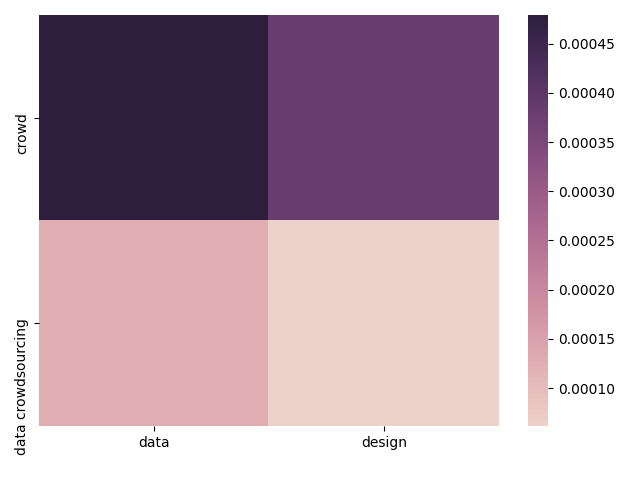
\includegraphics[width=400 pt]{output1.png}
  \caption{Figure 1.}
  \label{fig:matrix}
\end{figure}


\begin{figure}
  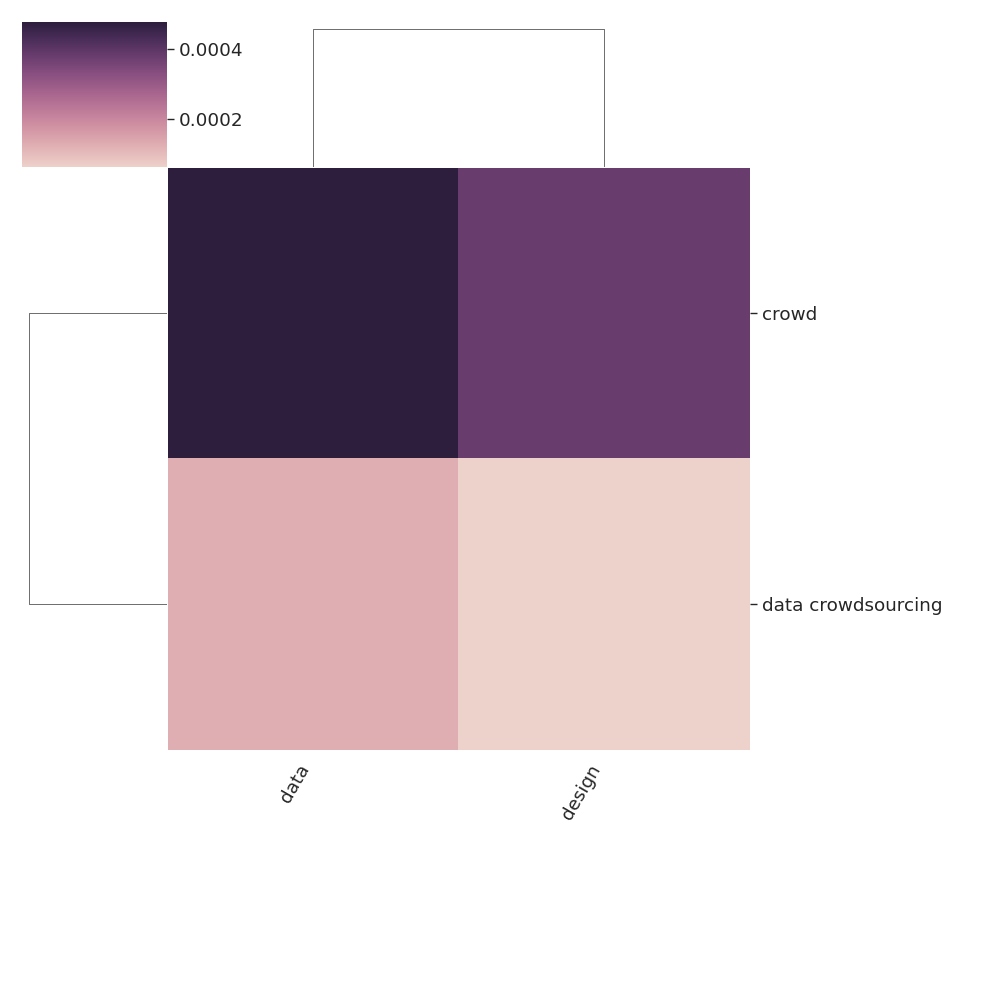
\includegraphics[width=\linewidth]{output2.png}
  \caption{Figure 2.}
  \label{fig:2}
\end{figure}



The words object provides a word cloud of the collected data for the first term (crowdsourcing), as shown in Figure~\ref{fig:3}.
\begin{figure}
  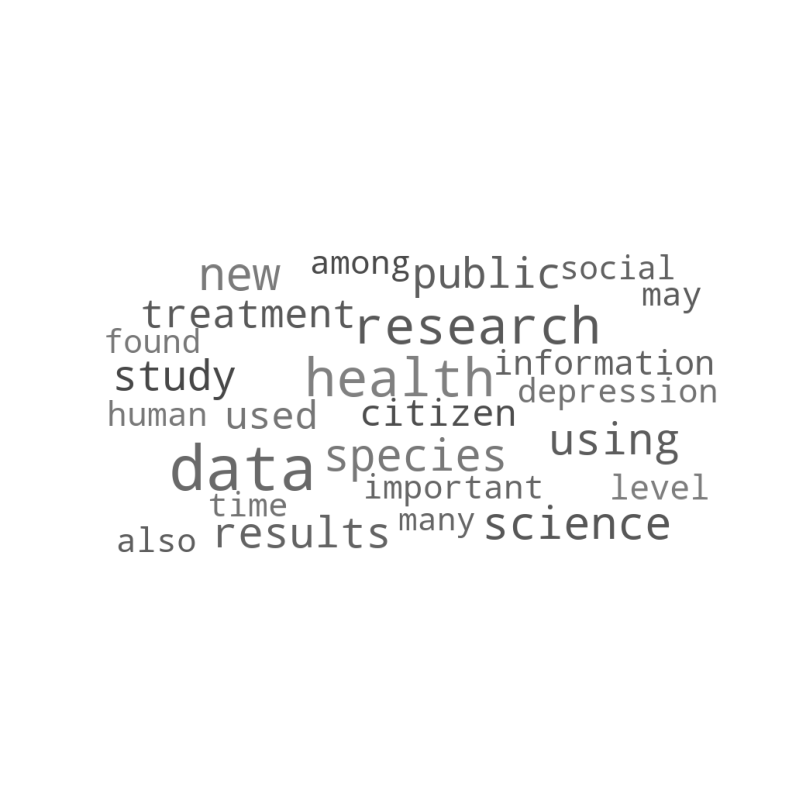
\includegraphics[width=\linewidth]{output3.png}
  \caption{Figure 3.}
  \label{fig:3}
\end{figure}

You can find more details about the articles' title, doi, and journal with this object.  Below is a sample output showing the titles of articles amongst 100 articles found by the term 'crowdsourcing' since 2018.

\VerbatimInput[frame=lines,numbers=left,numbersep=7pt,xrightmargin=0.5cm,resetmargins=true]{articles.txt}

\section{References}
 Donoghue, (2019). LISC: A Python Package for Scientific Literature Collection and Analysis. \emph{Journal of Open Source Software}, 4(41), 1674.
https://doi.org/10.21105/joss.01674
\newline
\newline
OpenCitations. (n.d.). OpenCitations. https://opencitations.net/
\newline
\newline
Sayers, E. (2020, August 6). \emph{A General Introduction to the E-utilities - Entrez Programming Utilities Help - NCBI Bookshelf}. The National Center for Biotechnology Information. https://www.ncbi.nlm.nih.gov/books/NBK25497/



\end{document}